\documentclass[10pt,border=2pt]{standalone}
\usepackage[T1]{fontenc}
\usepackage{lmodern}
\usepackage{pgfplots}
\pgfplotsset{compat=1.18}
\definecolor{convexblue}{HTML}{0072B2}
\definecolor{concaveorange}{HTML}{D55E00}
\begin{document}
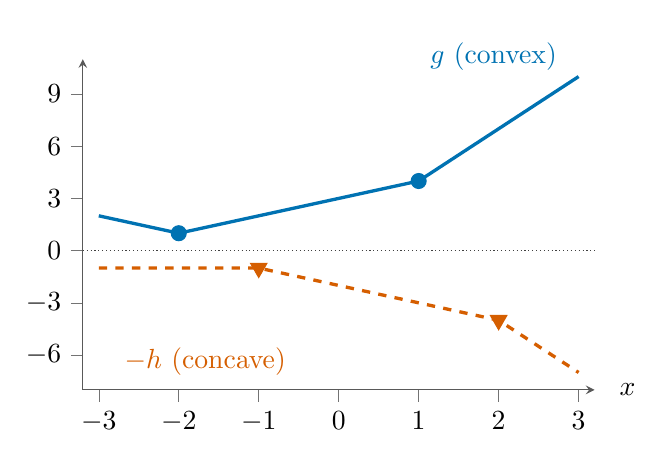
\begin{tikzpicture}
\path[use as bounding box] (-0.7,-0.65) rectangle (7.1,4.6);
\pgfplotsset{foldaxis/.style={
  scale only axis,width=6.5cm,height=4.2cm,
  at={(0,0)},anchor=south west,
  xmin=-3.2,xmax=3.2,xtick={-3,-2,-1,0,1,2,3},
  axis lines=left,axis line style={black!65},
  tick align=outside,tick style={black!55},
  xlabel={$x$},xlabel style={at={(axis description cs:1.03,0)},anchor=west},
  label style={font=\normalsize},tick label style={font=\normalsize},
  clip=false,
}}
\begin{axis}[foldaxis,ymin=-8,ymax=11,ytick={-6,-3,0,3,6,9}]
\addplot[black!75,densely dotted,thin] coordinates {(-3.2,0) (3.2,0)};
\addplot[convexblue,very thick] coordinates {(-3,2) (-2,1) (1,4) (3,10)};
\addplot[concaveorange,very thick,dashed] coordinates {(-3,-1) (-1,-1) (2,-4) (3,-7)};
\addplot[only marks,mark=*,mark size=2.7pt,convexblue] coordinates {(-2,1) (1,4)};
\addplot[only marks,mark=triangle*,mark options={rotate=180},mark size=3.4pt,concaveorange]
  coordinates {(-1,-1) (2,-4)};
\node[convexblue,anchor=south east] at (axis cs:2.85,9.8) {$g$ (convex)};
\node[concaveorange,anchor=west] at (axis cs:-2.8,-6.4) {$-h$ (concave)};
\end{axis}
\end{tikzpicture}
\end{document}
